% !TEX root = ../tex/1-2.tex
\begin{frame}{主要な深層生成モデリング}
    \begin{block}{生成モデリングにおける中心的な課題}
        \centering 高次元データの豊かで複雑な構造を捉えられる\\表現力の高い確率モデルの学習\\
    \end{block}
    \vspace{1em}
計算の扱いやすさ、表現力、学習効率の間で異なるトレードオフ\\
⇒代表的な戦略を紹介し、計算グラフの比較とともに説明する
\end{frame}
%========================================
\begin{frame}{1.2 Prominent Deep Generative Models}
    \begin{block}{定義:EBMs(Energy-based Models)}
        EBMs:エネルギー関数$\mathit{E}_{\phi}(x)$を通して確率分布を定義するモデル\\
        \centering{\Large $p_{\phi}(x):=\frac{1}{Z(\phi)}\exp(-\mathit{E}_{\phi}(x))$}\\
        \vspace{1em}
        ここで$Z(\phi)=\int \exp(-\mathit{E}_{\phi}(x))dx$は分配関数、
        これを代入すると\\
        {\Large$p_{\phi}(x)=\frac{\exp(-\mathit{E}_{\phi}(x))}{\int \exp(-\mathit{E}_{\phi}(x))dx}$}\\
        \begin{itemize}
            \item $exp(-\mathit{E}_{\phi}(x))>0$
            \item 分配関数で割ることで全体の積分が1になる
            \item もしxが離散変数なら$-E_{\phi}(x)$に対してソフトマックスを適用したものに近い\\
            ⇒連続変数の出力は確率密度なので1を越えてもいい。\\
            必要なのは全体の積分が1になること\\
        \end{itemize}
    \end{block}
\end{frame}
%========================================
\begin{frame}{}
    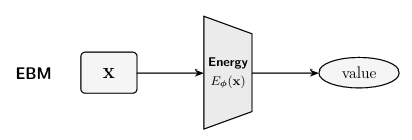
\includegraphics[
        width=\textwidth,
        height=0.78\textheight,
        keepaspectratio
    ]{figure1-2.png}
    \begin{exampleblock}{}
    エネルギー関数:高次元データxに対して1つの実数$\mathit{E}_{\phi}(x)$を割り当てている
    ($\mathit{E}_{\phi}(x):R^D \rightarrow R$)\\
    $\mathit{E}_{\phi}(x)$は正規化定数が有限の範囲内で柔軟に設計可能\\
    実数全体で$E_{\phi}(x)=0 \implies Z=\int_{-\infty}^{\infty} 1dx=\infty$より正規化できない\\
\end{exampleblock}
EBMを通してエネルギー→確率密度の変換を行っている\\
    
    EBMの学習ではデータの対数尤度を最大化する\\
    しかし、分配関数が計算困難で対処が必要\\
    ⇒次の章で拡散モデルについて解説
\end{frame}

%========================================
\begin{frame}{AutoRegressive Models}
    \begin{block}{定義:AutoRegressive Models(自己回帰モデル)}
    ARモデル:各データ点が前のデータ点に依存して生成されるモデル\\
\end{block}
    これは確率の連鎖率を用いることで、どんな同時分布も一連の条件付確率に分解が可能\footnote{chain rule:next slide}\\
    変数$x=(x_1,x_2,\ldots,x_d)$に対して、$p_{data}(x)=\prod_{i=1}^d p(x_i|x_{<i}),x_{<i}=x_1,\ldots,x_{i-1}$と表せる\\
    (モデル化の仮定ではなく変数について順不同の厳密な恒等式)\\
    \vspace{1em}
    問題は$p_{data}(x_{i}\mid\boldsymbol{x}_{<i})$が未知であること\\
    ⇒ARモデルは同じ因数分解の形を持つモデルをパラメータ化\\
    $\log p_{\phi}(\mathit{x})=\sum_{i=1}^{D}\log p_{\phi}(x_{i}\mid\boldsymbol{x}_{<i})$
\end{frame}
%=============================================
\begin{frame}{AutoReguression Models}

    \begin{exampleblock}{NNの出力(e.x.語彙生成)⇒条件付分布の近似}
        モデルに系列トークンを入力し、次のトークンの確率分布を出力\\
        \vspace{1em}
        入力に対し次トークンの候補を数値化し、softmaxで確率に変換\\
        {\centering $p_{\phi}(x_{i}=k\mid\boldsymbol{x}_{<i})=\frac{\exp(a_{k})}{\sum_{k'\in \mathcal{V}}\exp(a_{k'})}$\par}
        \begin{itemize}
            \item 確率は非負で候補全体の総和が1
            \item $a_{k}$は前の要素$x_{<i}$とパラメータ$\phi$によって変わる
        \end{itemize}
        連続値の場合、正規化分布の平均と標準偏差を出力し、\\
        $p_{/phi}(x_{i}\mid x_{<i})=\mathcal{N}(\mu_{\phi}(x_{<i}),\sigma_{\phi}(x_{<i})^2)$
        \vspace{1em}
        \begin{itemize}
            \item 各位置に別々のネットワークが必要とは限らない
            \item 全ての位置で同じパラメータを使うことも可能
            \item 入力される前の要素に応じて異なる条件付分布を出力可能
        \end{itemize}
    \end{exampleblock}
\end{frame}
%======================================
\begin{frame}{AutoReguression Models}
    \begin{alertblock}{なぜ積をとるだけで全体が正規化されるのか}
        三つの離散変数の場合\\
        $p_{data}(x_1,x_2,x_3)=p_{data}(x_1\mid x_2,x_3)p_{data}(x_2\mid x_3)p_{data}(x_3)$\\
        全ての値について足すと\\
        $\sum_{x1}p_{\phi}(x_{1})\sum_{x2}p_{\phi}(x_{2}\mid x_{1})\sum_{x3}p_{\phi}(x_{3}\mid x_{1},x_{2})=1$\\
        最後の変数から順に足していくと条件付分布の総和が1になり、全体も1になる。連続なら和を積分に置き換える\\
    \end{alertblock}
    EBMではデータ空間全体の正規か定数が問題\\
    ⇒ARモデルでは全体正規化が保証される
\end{frame}
%======================================
\begin{frame}{学習について}
    \begin{block}{尤度に基づく学習が容易になる}
    データサンプル$\mathit{x}^{(1)},...,\mathit{x}^{(N)}$に対応する対数尤度は\\
    $\log p_{\phi}(\mathit{x})=\sum_{i=1}^{D}\log p_{\phi}(\mathit{x}_i\mid\mathit{x}_{<i})$のように分解される\\
    \vspace{1em}
    \begin{itemize}
    \item 最尤推定によって直接学習可能\\
    ⇒これは負の対数尤度を最小かすることと同値\\
    \vspace{1em}
    \item 観測済みの先行変数$x_{<i}$が利用できる\\⇒
    条件付き予測の並列計算が可能
    \end{itemize}
    \end{block}


\end{frame}
%======================================
\begin{frame}{生成について}
    \begin{block}{生成は逐次的に行われる}
    生成では正解の列がないためまず一つ目を生成する\\
    $x_1 \sim p_{\phi}(x_1)$\\
    その結果を使って\\
    $x_2 \sim p_{\phi}(x_2\mid x_1)$\\
    これを繰り返していくことで生成が可能\\
    ⇒次の分布を決める条件が前の生成結果に依存する
    \end{block}
    ここでの生成は最も確率が高い候補を選ぶということではなく\\
    分布からランダムにサンプリングする\\
    ⇒同じ条件で異なるデータを生成可能
\end{frame}
%=============================================
\begin{frame}{VAE:variational Autoencoder}
    \begin{block}{VAE(変分オートエンコーダ)}
        VAE:データに隠れた構造である潜在変数$\mathit{z}$を学習するモデル\\
        (オートエンコーダの拡張)\\
        $\mathit{x}と\mathit{z}$間の写像を直接学習する代わりに確率的な見方を採用する\\
        エンコーダとデコーダの両方を学習する\\
        \begin{itemize}
            \item エンコーダ$q_{\theta}(\mathit{z}\mid\mathit{x})$:\\
            ⇒データが与えられたときの潜在変数の未知の分布を近似
            \item デコーダ$p_{\phi}(\mathit{x}\mid\mathit{z})$:\\
            ⇒潜在変数からデータを再構成する
        \end{itemize}
    \end{block}
    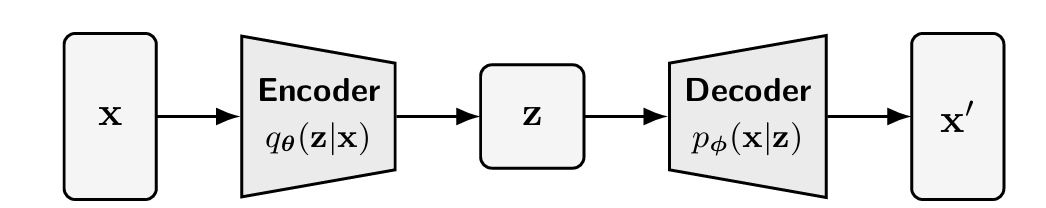
\includegraphics[
        width=\textwidth,
        height=0.78\textheight,
        keepaspectratio
    ]{AutoEncoder.png}
\end{frame}
%======================================
\begin{frame}{AE(AutoEncoder)}
    \begin{exampleblock}{AEとVAEの違い}
    \begin{itemize}
    \item 学習するもの\\
    AE:入力を復元する写像\\
    VAE:潜在変数を介してデータを生成する確率モデル\\


    \end{itemize}
    \end{exampleblock}

\end{frame}
%======================================
\begin{frame}{ELBO(Evidence Lower Bound)}
    \begin{block}{ELBO(Evidence Lower Bound)}
        $\mathit{L}_{\mathit{ELBO}}(\theta,\phi;x)=\mathbb{E}_{z\sim q_{\theta}(\mathit{z}\mid\mathit{x})}[\log p_{\phi}(\mathit{x}\mid\mathit{z})]-\mathit{D}_{KL}(q_{\theta}(\mathit{z}\mid\mathit{x})\mid\mid p(\mathit{z}))$\\
        \vspace{1em}
        真の対数尤度の代わりに計算可能なエビデンス下界を最大化する\\
        \vspace{1em}
        第一項はデータの正確な再構成を促す項\\
        第二項は潜在変数の分布$p_{perior}(\mathit{z})$を単純な事前分布に近づけ、正則化する項\\
    \end{block}
    【VAEについて】\\
    ニューラルネットワークと潜在変数モデルを組み合わせる方法で\\
    尤度に基づくアプローチとして最も多く使われている一つの手法\\
    \vspace{1em}
    生成サンプルの鮮明さが不十分、学習上の問題などの実用上の\\課題がありつつも拡散モデルなどの発展の基礎となっている

\end{frame}
%======================
\begin{frame}{ELBOの導出}
    \begin{exampleblock}{}
        対数尤度に潜在変数$\mathit{z}$における任意の分布$q(\mathit{z})$を用いて
            \begin{align*}
        \log p_{\theta}(\mathbf{x}) &= \log p_{\theta}(\mathbf{z}\mid\mathbf{x})\int q(\mathit{z})d\mathbf{z}\\
        &=\int q(\mathit{z})\log p_{\theta}(\mathbf{x})d\mathbf{z}\\
        &=\int q(\mathit{z})\log \frac{q(\mathit{z})p_{\theta}(\mathbf{z}, \mathit{x})p_{\theta}(\mathbf{x})}{q(\mathit{z})p_{\theta}(\mathbf{z}\mid\mathbf{x})}d\mathbf{z}\\
        &=\int q(\mathit{z})\log \frac{p_{\theta}(\mathbf{z}, \mathit{x})p_{\theta}(\mathbf{x})}{q(\mathit{z})}d\mathbf{z}
        +\int q(\mathit{z})\log \frac{q(\mathit{z})}{p_{\theta}(\mathbf{z}\mid\mathbf{x})}d\mathbf{z}\\
        &=\mathit{L}(\theta,\phi;x)+\mathit{D}_{KL}(q(\mathit{z})\mid\mid p_{\theta}(\mathbf{z}\mid\mathbf{x}))
    \end{align*}
    ただし$\mathit{L}(\theta,\phi;x)=\int q(\mathit{z})\log \frac{p_{\theta}(\mathbf{z}, \mathit{x})}{q(\mathit{z})}d\mathbf{z}$\\
    第一項はELBO、第二項はKLダイバージェンス\\
    第二項は0以上なのでELBOは必ず周辺尤度の下界を与える$log p_{\theta}(\mathbf{x})\geq \mathit{L}(\theta,\phi;x)$
    \end{exampleblock}
\end{frame}
%======================================
\begin{frame}{Nomalization Flows}
    \begin{block}{従来の正規化フロー：}
    正規化フロー(NF)とニューラル常微分方程式(NODE)に基づく\\
    連続時間のモデル\\
    ⇒可逆の変換を用いて、単純な潜在変数と複雑なデータの分布を結び付ける全単射を学習\\
    $\log p_{\phi}(x)=\log p(f_{\phi}(x))+\log\left|\det\frac{\partial f_{\phi}(x)}{\partial x}\right|,$
    $z=f_{\phi}(x),x=f_{\phi}^{-1}(z)$\\
    \end{block}
    概念的には美しいが、実装上の制約が多い\\
    \begin{itemize}
        \item 全単射を保証するためネットワーク構造に厳しい制約
        \item 常微分方程式を解く計算負荷が高く学習効率低下
        \item 可逆で、ヤコビアンの行列式も効率よく計算できる変換
    \end{itemize}
\end{frame}
%======================================
\begin{frame}{解釈}
    \begin{exampleblock}{\small 目的：実際のデータに近い分布を学習し、新しいデータを生成\\}
        \small 分布から得たサンプル(z)は潜在変数であり高次元のベクトル\\
        潜在変数を変換して実際のデータに近い形にする\\
        ※ここで、生成されたxの確率密度が計算できるとは限らない\\
        ⇒可逆な変換によって潜在変数zの確率密度を使えるようにする\\
        $z=f_{\phi}(x),x=f_{\phi}^{-1}(z)$\\
        \vspace{1em}
        ただし、変換によって空間が伸び、単位体積当たりの確率密度が変わるので対数変換の公式を用いて対策する\\
        $p_{\phi}(x)=p(f_{\phi}(x))\left|\det\frac{\partial f_{\phi}(x)}{\partial x}\right|,$\\
        対数をとって
        $\log p_{\phi}(x)=\log p(f_{\phi}(x))+\log\left|\det\frac{\partial f_{\phi}(x)}{\partial x}\right|$\\
        \vspace{1em}
        学習データを大きくするように、パラメータ \(\phi\) を学習可能になる\\
        ⇒「変数変換の公式によって最尤推定が可能になる」
    \end{exampleblock}
\end{frame}
%======================================
\begin{frame}{GANs:Generative Advasarial Networks}
    \begin{block}{GANs:Generative Advasarial Networks}
        GANs:生成器$\mathit{G}$と判別機$\mathit{D}$が互いに競い合う二つのNN\\
        \begin{itemize}
        \item 生成器$\mathit{G}$:ランダムなノイズ$\mathit{z}\sim P_{prior}$から\\現実的なサンプル$\mathit{G}_{\phi}(z)$を作ることを目指す
        \item 判別機$\mathit{D}$:実サンプル$\mathit{x}$か生成サンプル$\mathit{G}_{\phi}(z)$かを判別する
        \end{itemize}
        GANsの目的関数:\\
        \[\min_{G_\phi}\max_{D_\zeta}\left\{\underbrace{\mathbb{E}_{x\sim p_{\mathrm{data}}}[\log D_\zeta(x)]}_{\text{実サンプル}}+\underbrace{\mathbb{E}_{z\sim p_{\mathrm{prior}}}\left[\log\left(1-D_\zeta(G_\phi(z))\right)\right]}_{\text{生成サンプル}}\right\}.\]
        \begin{itemize}
            \item 明示的な確率密度関数を定義しない⇒尤度の推定を回避\\
            \item 正規化定数を計算せず、よく模倣するサンプルの生成に重点\\
        \end{itemize}
    \end{block}
\end{frame}
%======================================
\begin{frame}{ダイバージェンスの観点から見ると}
    \begin{exampleblock}{}
        \small $\mathit{D_\zeta}$が真の分布 \(p_{\mathrm{data}}\) と生成器の分布 \(p_{G_\phi}\) の間の隔たりを暗黙的に測る\\
        ※\(p_{G_\phi}\) は、ノイズ \(z\sim p_{\mathrm{prior}}\) から得られる生成サンプル \(G_\phi(z)\) の分布
        生成器 \(G_\phi\) を固定したとき、最適な識別器は\\
        \[D^*(x)=\frac{p_{\mathrm{data}}(x)}{p_{\mathrm{data}}(x)+p_{G_\phi}(x)}\]\\
        この最適な最適な識別機を用いると生成器の最小化問題は\\
        \[\min_{G_\phi}\left[2D_{\mathrm{JS}}(p_{\mathrm{data}}\|p_{G_\phi})-\log 4\right]\]\\
        ここで\(D_{\mathrm{JS}}\) は次のように定義される\\
        \[D_{\mathrm{JS}}(p\|q):=\frac12D_{\mathrm{KL}}\left(p\middle\|\frac{p+q}{2}\right)+\frac12D_{\mathrm{KL}}\left(q\middle\|\frac{p+q}{2}\right).\]
        GANが暗黙的に \(D_{\mathrm{JS}}(p_{\mathrm{data}}\|p_{G_\phi})\) を最小化していることを示している\\
    \end{exampleblock}
\end{frame}

%======================================
\begin{frame}{chain rule}
    \begin{block}{chain rule:確率の連鎖律(確率の乗法定理)}
        複数の確率変数の同時確立を条件付確率の積として表す公式\\
        イメージ：
        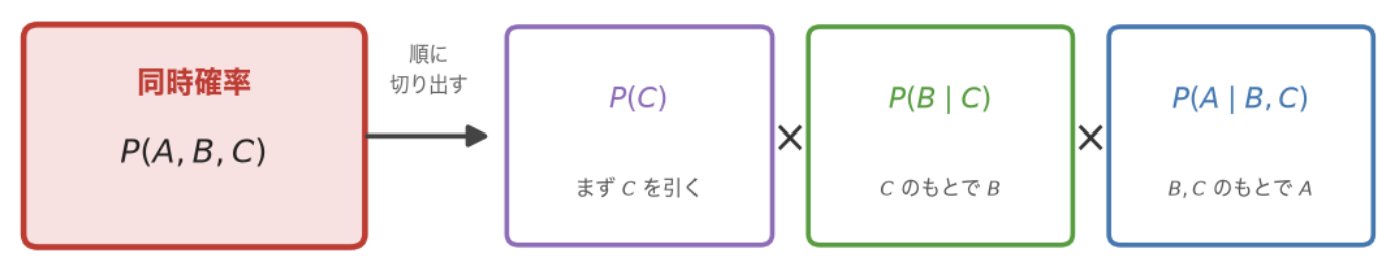
\includegraphics[
        width=\textwidth,
        height=0.78\textheight,
        keepaspectratio
    ]{chainrule.png}
    条件付確率$P(A\mid B)=\frac{P(A,B)}{P(B)}$\\
    両辺に$P(B)$をかけると$P(A,B)=P(A\mid B)P(B)$\\
    \end{block}
    \begin{exampleblock}{3変数の場合}
        $P(A,B,C)=P(A\mid B,C)P(B\mid C)P(C)$\\
        ここで$P(B,C)$は2変数の同時確立なのでもう一度乗法定理\\
        $P(B,C)=P(B\mid C)P(C)$より\\
        $P(A,B,C)=P(A\mid B,C)P(B\mid C)P(C)$\\
    \end{exampleblock}
\end{frame}
%======================================
\begin{frame}{chain ruleの一般化}
    \begin{block}{chain ruleの一般化}
        n個の確率変数$A_{1},A_{2},...,A_{n}$の同時確率からまず$A_{1}$を切り出すと\\
        $P(A_{1},A_{2},...,A_{n})=P(A_{1}\mid A_{2},...,A_{n})P(A_{2},A_{3},...,A_{n})$\\
        ここで$P(A_{2},A_{3},...,A_{n})$はn-1個の確率変数の同時確率なので\\
        もう一度乗法定理によって\\
        $P(A_{1},A_{2},...,A_{n})=P(A_{1}\mid A_{2},...,A_{n})...P(A_{n-1}\mid A_{n})P(A_{n})$\\
        したがって\\
        {\centering $P(A_{1},A_{2},...,A_{n})=\prod_{i=1}^{n}P(A_{i}\mid A_{i+1},...,A_{n})$\par}
        \vspace{1em}
        ※最初の項は$P(A_{1})$になる\\
    \end{block}
    どの変数にも対称に使え、別の順序でも同じ同時確率が得られる\\
    ⇒問題ごとに計算しやすい順序を選べる
\end{frame}
%======================================